%%%%%%%%%%%%%%%%%%%%%%%%%%%%%%%%%%%%%%%%%%%%%%%%%%%%%%%%%%%%%%%%%%%%%%%%
%    INSTITUTE OF PHYSICS PUBLISHING                                   %
%                                                                      %
%   `Preparing an article for publication in an Institute of Physics   %
%    Publishing journal using LaTeX'                                   %
%                                                                      %
%    LaTeX source code `ioplau2e.tex' used to generate `author         %
%    guidelines', the documentation explaining and demonstrating use   %
%    of the Institute of Physics Publishing LaTeX preprint files       %
%    `iopart.cls, iopart12.clo and iopart10.clo'.                      %
%                                                                      %
%    `ioplau2e.tex' itself uses LaTeX with `iopart.cls'                %
%                                                                      %
%%%%%%%%%%%%%%%%%%%%%%%%%%%%%%%%%%
%
%
% First we have a character check
%
% ! exclamation mark    " double quote
% # hash                ` opening quote (grave)
% & ampersand           ' closing quote (acute)
% $ dollar              % percent
% ( open parenthesis    ) close paren.
% - hyphen              = equals sign
% | vertical bar        ~ tilde
% @ at sign             _ underscore
% { open curly brace    } close curly
% [ open square         ] close square bracket
% + plus sign           ; semi-colon
% * asterisk            : colon
% < open angle bracket  > close angle
% , comma               . full stop
% ? question mark       / forward slash
% \ backslash           ^ circumflex
%
% ABCDEFGHIJKLMNOPQRSTUVWXYZ
% abcdefghijklmnopqrstuvwxyz
% 1234567890
%
%%%%%%%%%%%%%%%%%%%%%%%%%%%%%%%%%%%%%%%%%%%%%%%%%%%%%%%%%%%%%%%%%%%
%
\documentclass[12pt]{article}
\newcommand{\gguide}{{\it Preparing graphics for IOP Publishing journals}}
%Uncomment next line if AMS fonts required
%\usepackage{iopams}
\usepackage{graphicx}
\usepackage{hyperref}   % to set up hyperlinks
\hypersetup{
	colorlinks=true,
	linkcolor=blue,
	citecolor=blue,
	urlcolor=blue,
}

\begin{document}

%%\note{A novel passive
%%ferrofluid check (one-way) valve}

\title{A Novel Passive Ferrofluid One-way (Check) Valve}


%%% first author
\author{Robert L. Read}

\begin{abstract}

  Currently this is very preliminary. This is an attempt to design a pump that can efficiently pump ferrofluid with no moving parts
  except the ferrofluid and two blobs of an immiscible, incompressible fluid, such as water.
  Eliminating moving parts allows miniaturization and potentially fabrication as a chip.
  A miniature pump could be used for cooling a chip and for ``lab on a chip'' applications.
  The proposed design uses two permanent magnets and seven controllable electromagnets.
  The design was developed from considering the minimal topological connection of fixed chambers.
  It has four distinct phases, each phase having a distinct magnetic configuration.
\end{abstract}

%
% Uncomment for keywords
\vspace{2pc}
\noindent{\it Keywords}: ferrofluid pump

% Uncomment if a separate title page is required
%\maketitle
%
% For two-column output uncomment the next line and choose [10pt] rather than [12pt] in the \documentclass declaration
%\ioptwocol
%


%%%%%%%%%%%%%%%%%%%%%%%%%%%%%%%%%%%%%%%%%%%%%%%%%%%%%%%%%%%%%%%%%%%%%%
\section{Introduction}

Ferrofluid can be manipulated by electronically controlled magnetic
fields to exert force on fluids\cite{torres2014recent,kole2021engineering,ozbey2015modeling}.
This makes it possible to build pneumatic or hydraulic
devices, perhaps on very small scales,
such as a single chip\cite{yamahata2003ferrofluid,hatch2001ferrofluidic}, to
miniaturize fluid handling.
This has been proposed for biomedical purposes\cite{michelson2019novel}
that would use water or body fluids,
although this paper reports only on experiments done with air.
Miniature pumps and valves could be used to make a “lab on a chip” (LOC) or
even to heat or cool different chip areas.

%%%%%%%%%%%%%%%%%%%%%%%%%%%%%%%%%%%%%%%%%%%%%%%%%%%%%%%%%%%%%%%%%%%%%%
\section{Related Research}

A number of papers report on ferrofluid pumps, focusing in particular
on micropump and lab-on-a-chip applications\cite{ozbey2015modeling,hsu2018biocompatible}.
Many of these papers use
a version of mechanical valve not based on passive
ferrofluid, even though they move a ferrofluid bolus
with a magnetic field.
For example,
a corrugated silicone micro valve\cite{yamahata2003ferrofluid,yamahata2005plastic}
has been reported.
Other researchers use active valves, which require synchronization with
the ferrofluid plug to form a pump,
such as \cite{menz2000fluidic}, which
describes an active {\em T-Valve} with a moving ferrofluid plug, and
\cite{ando2009ferrofluidic} describes a complete fluid pump with valves
that use
active control of a ferrofluid bolus.
At least two additional kinds of active valves, a {\em well valve} and
{\em Y-valve}, have
been described\cite{hartshorne2004ferrofluid}.
Active control is possible because the
action of the plunger or bolus may be synchronized with the opening and closing
of the valves.
Nonetheless a passive valve would be simpler and less
expensive, and would not require knowledge of the timing of the
plunger.

An interesting functional micropump in which the
moving ferrofluid bolus merges with a fixed ferrofluid valve and then
separates on each pumping cycle has been described\cite{hatch2001ferrofluidic}.

An interesting devices induces a flow directly in ferrofluid
with no moving parts,
presumable based on the rotation of clumps of ferrofluid
\cite{mao2011direct}.

\section{The Idea}

There is no known way to directly move a mass of ferrfluid which is immersed in
ferrofluid.
The idea of moving a ferrofluid plug or bolus which is bouneded by air or water
via electromagnets turned on or off is well known. A slight inversion of this
idea is to use two boluses to trap a blob of water. The water thus remains
a separator. In the diagrams below it is represented as a ``W'',
and the ferrofluid as an ``F''.
The separator allows us to move the bolus slightly.
In order to create a pump, we need to recycle this separator, rather than
moving it once, as in a piston.

If we combine this with the idea of a moving bolus ``picking up'' some ferrofluid
and then dropping some of that ferrofluid, we can have a two circulating water blobs
and two circulating ferrofluid plugs. One ferrofluid plug, which is moving from the
inlet to the outlet, is larger.
The other plug is smaller, and merely separating the water plugs as it is returned.

If we reduce this to a minimal configuration, we have a circle of seven regions
of equal size. The inlet and the outlet prevent the water blobs from escaping by
having permanent magnets in place. The water blobs can never displace these
locks, represented by ``L'' in our diaggram. The inlet of the pump has an
inexhaustible supply of ferrofluid represented as a source (``S''). The
outlet is represented as a drain ``D''.

The water plugs must always be kept separated by ferrofluid plugs. However,
these plugs can pull fluid from the source and push it into the drain if
so driven by the changing magnets in the seven dynamic regions.
By cycling through four configurations as depicted, we can move ferrofluid
from the source to the drain.




\begin{figure}
\centerline{
\includegraphics[width=5in]{images/Ferrofluid Pump.png}}
\caption{The Pump Schematic}
\label{fig_pumpschematic}
\end{figure}

\begin{figure}
\centerline{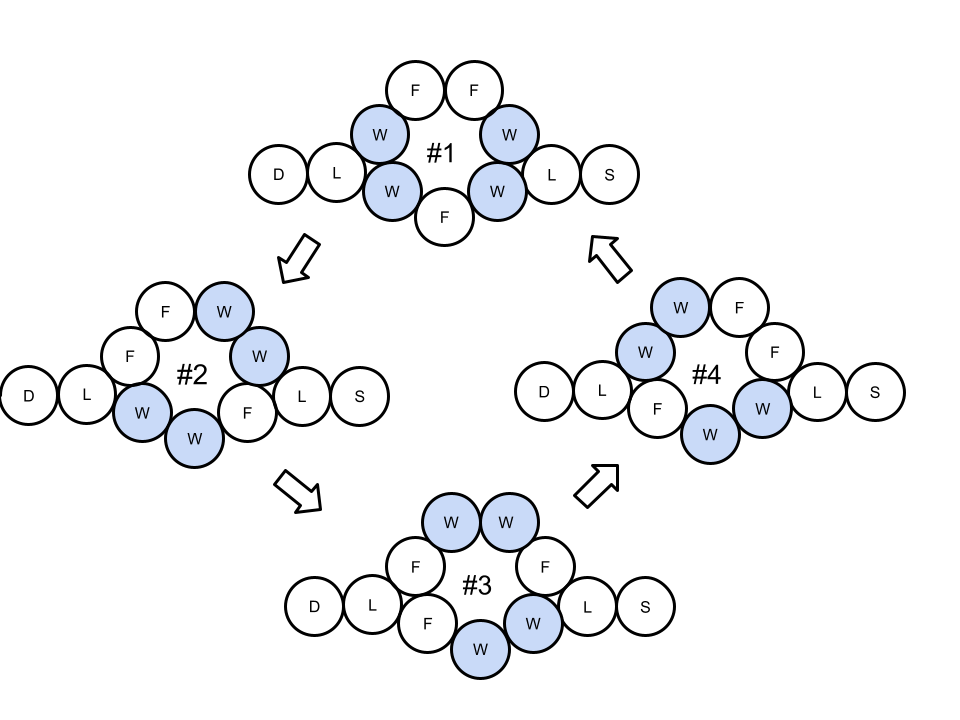
\includegraphics[width=5in]{images/PumpPhases.png}}
\caption{The Pump Schematic}
\label{fig_pumpschematic}
\end{figure}


\section{Conclusions}

\section{TODO}

Study this: \url{http://citeseerx.ist.psu.edu/viewdoc/download?doi=10.1.1.719.4343&rep=rep1&type=pdf}

\section{Acknowledgements}

This paper was an outgrowth the the Passive Ferrrofluid Check Valve (PFCV) \cite{stuckeynovel}
reported by Veronica Stuckey and Robert L. Read. Veronica Stuckery 3D printed
some of the apparatus.

\section*{References}

\bibliographystyle{unsrt}
% Here's where you specify the bibliography database file.
% The full file name of the bibliography database for this
% article is asme2e.bib. The name for your database is up
% to you.
\bibliography{ffcv}

\end{document}
